%============================================================
%  MẪU CHUẨN SOẠN ĐỀ EDUZY (ex_test v3.3)
%  - Phần KHUNG (từ \def\CheDo đến các \subsection*, \setcounter, \Opensolutionfile)
%    chỉ dùng khi biên dịch hoặc khi bật công tắc "khung đề".
%  - Các khối \begin{ex}...\end{ex} và \begin{bt}...\end{bt} là ĐÚNG định dạng
%    đầu ra cần trả về trong chat.
%  - Các biến thể theo công tắc (chỉ đề, choiceTF, mã dạng) để dạng comment ở cuối file.
%============================================================
\def\CheDo{loigiai}% loigiai | dethi
\def\tenchuong{Mẫu chuẩn soạn đề -- Eduzy}
\input{preamble-eduzy}
\begin{document}
	\khungtieude{THI THỬ THPT QUỐC GIA NĂM 2026}{Môn Toán -- Đề mẫu}{(Đề thi gồm: 12 câu trắc nghiệm, 04 câu đúng-sai, 06 câu trả lời ngắn)}{Thời gian làm bài: 90 phút (không kể thời gian phát đề).}
	
	\noindent
	\subsection*{\indam{PHẦN I. Câu trắc nghiệm nhiều phương án lựa chọn. Thí sinh trả lời từ câu 1 đến câu 12. Mỗi câu hỏi thí sinh chỉ chọn một phương án.}}
	\setcounter{ex}{0}
	\Opensolutionfile{ans}[ans/Mau-1]
	
	%--- Trắc nghiệm 4 phương án, không hình
	\begin{ex}
		Trong không gian với hệ tọa độ $Oxyz$, cho mặt phẳng $(P)\colon x-2y+2z-1=0$. Một vectơ pháp tuyến của mặt phẳng $(P)$ có tọa độ là
		\choice
		{\True $(1;-2;2)$}
		{$(-1;1;2)$}
		{$(-1;-2;2)$}
		{$(1;2;2)$}
		\loigiai{
			Mặt phẳng $(P)\colon x-2y+2z-1=0$ có một vectơ pháp tuyến là $\overrightarrow{n}=(1;-2;2)$.
		}
	\end{ex}
	
	%--- Đồ thị hàm số bằng pgfplots, đặt giữa bằng center, trước \choice
	\Needspace{16\baselineskip}
	\begin{ex}
		Cho hàm số $y=f(x)$ có đồ thị như hình vẽ. Tổng của giá trị lớn nhất và giá trị nhỏ nhất của hàm số đã cho trên đoạn $[-2;2]$ bằng
		\begin{center}
			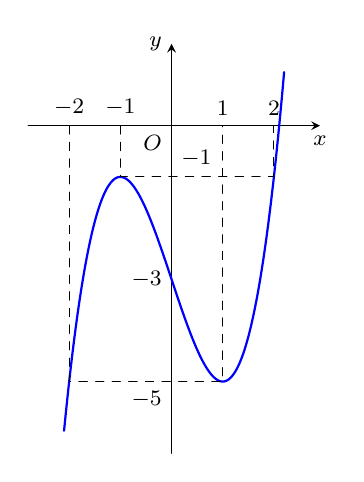
\begin{tikzpicture}[line join=round,line cap=round,>=stealth,font=\footnotesize]
				\begin{axis}[x=0.65cm,y=0.65cm,
					axis lines=middle,axis line style={->},
					xmin=-2.8,xmax=2.9,ymin=-6.4,ymax=1.6,
					xtick=\empty,ytick=\empty,
					xlabel={$x$},ylabel={$y$},
					xlabel style={anchor=north},ylabel style={anchor=east},
					clip=false]
					\addplot[thick,blue,smooth,samples=100,domain=-2.1:2.2]{x^3-3*x-3};
					\draw[dashed] (-2,0)--(-2,-5)--(1,-5)--(1,0);
					\draw[dashed] (-1,0)--(-1,-1)--(2,-1)--(2,0);
					\pgfplotsinvokeforeach{-2,-1,1,2}{\node[above] at (#1,0){$#1$};}
					\node[below left] at (0,0){$O$};
					\node[above right] at (0,-1){$-1$};
					\node[left] at (0,-3){$-3$};
					\node[below left] at (0,-5){$-5$};
				\end{axis}
			\end{tikzpicture}
		\end{center}
		\choice
		{$-1$}
		{\True $-6$}
		{$0$}
		{$-5$}
		\loigiai{
			Từ đồ thị, ta có $\max\limits_{[-2;2]}f(x)=f(-1)=f(2)=-1$ và $\min\limits_{[-2;2]}f(x)=f(-2)=f(1)=-5$.\\
			Vậy tổng cần tìm là $-1+(-5)=-6$.
		}
	\end{ex}
	
	%--- Bảng xét dấu / bảng biến thiên bằng tkz-tab
	\begin{ex}
		Cho hàm số $y=f(x)$ có đạo hàm trên $\mathbb{R}$ và có bảng xét dấu của $f'(x)$ như sau:
		\begin{center}
			
\begin{tikzpicture}
				\tkzTabInit[lgt=1.5,espcl=2,deltacl=0.6]{$x$/0.8,$f'(x)$/0.8}{$-\infty$,$-3$,$1$,$2$,$+\infty$}
				\tkzTabLine{,-,z,+,z,+,z,-,}
			\end{tikzpicture}
		\end{center}
		Số điểm cực trị của hàm số $y=f(x)$ là
		\choice
		{$3$}
		{$1$}
		{\True $2$}
		{$0$}
		\loigiai{
			$f'(x)$ đổi dấu khi $x$ đi qua $x=-3$ và $x=2$, không đổi dấu khi $x$ đi qua $x=1$ nên hàm số đã cho có $2$ điểm cực trị.
		}
	\end{ex}
	
	%--- Hệ phương trình: \left\{\begin{aligned}...\end{aligned}\right.
	\begin{ex}
		Nghiệm $(x;y)$ của hệ phương trình $\left\{\begin{aligned}&2x+y=5\\&x-y=1\end{aligned}\right.$ là
		\choice
		{\True $(2;1)$}
		{$(1;2)$}
		{$(3;-1)$}
		{$(2;-1)$}
		\loigiai{
			Cộng vế theo vế hai phương trình, ta được $3x=6\Leftrightarrow x=2$. Suy ra $y=x-1=1$.\\
			Vậy hệ có nghiệm $(x;y)=(2;1)$.
		}
	\end{ex}
	
	%--- Hình không gian bằng TikZ thuần (không tkz-euclide)
	\Needspace{14\baselineskip}
	\begin{ex}
		Cho hình hộp $ABCD.A'B'C'D'$ (\textit{tham khảo hình vẽ}). Khi đó, tổng $\overrightarrow{AB}+\overrightarrow{AD}+\overrightarrow{DD'}$ bằng
		\begin{center}
			\begin{tikzpicture}[scale=0.7,line join=round,line cap=round,font=\footnotesize]
				\coordinate (B) at (0,0);
				\coordinate (C) at (4,0);
				\coordinate (A) at (1.4,1);
				\coordinate (D) at ($(A)+(C)-(B)$);
				\coordinate (B') at (0,2.2);
				\coordinate (C') at ($(C)+(B')-(B)$);
				\coordinate (A') at ($(A)+(B')-(B)$);
				\coordinate (D') at ($(D)+(B')-(B)$);
				\draw (B)--(C)--(C')--(B')--cycle (B')--(A')--(D')--(C') (C)--(D)--(D');
				\draw[dashed] (B)--(A)--(D) (A)--(A');
				\foreach \p/\pos in {A/left,B/below left,C/below right,D/right,A'/above left,B'/left,C'/above left,D'/above right}
				\node[\pos] at (\p){$\p$};
			\end{tikzpicture}
		\end{center}
		\choice
		{$\overrightarrow{C'A}$}
		{\True $\overrightarrow{AC'}$}
		{$\overrightarrow{AD'}$}
		{$\overrightarrow{D'A}$}
		\loigiai{
			Vì $\overrightarrow{DD'}=\overrightarrow{AA'}$ nên theo quy tắc hình hộp, ta có
			\[
			\overrightarrow{AB}+\overrightarrow{AD}+\overrightarrow{DD'}=\overrightarrow{AB}+\overrightarrow{AD}+\overrightarrow{AA'}=\overrightarrow{AC'}.
			\]
		}
	\end{ex}
	
	\Closesolutionfile{ans}
	
	\subsection*{\indam{PHẦN II. Câu trắc nghiệm đúng sai. Thí sinh trả lời từ câu 1 đến câu 4. Trong mỗi ý a), b), c), d) ở mỗi câu, thí sinh chọn đúng hoặc sai.}}
	\setcounter{ex}{0}
	\Opensolutionfile{ans}[ans/Mau-2]
	
	%--- Đúng/Sai: \choiceTFt, lời giải bằng itemchoice
	\begin{ex}
		Cho hàm số $f(x)=\dfrac{2x+4}{x-1}$.
		\choiceTFt
		{\True Tổng số đường tiệm cận ngang và tiệm cận đứng của đồ thị hàm số là $2$}
		{Tâm đối xứng của đồ thị hàm số là $I(2;1)$}
		{Hàm số đã cho có hai điểm cực trị}
		{\True $\max\limits_{[-2;0]}f(x)=0$}
		\loigiai{
			\begin{itemchoice}
				\itemch {\bf Đúng.}\\
				Tập xác định $D=\mathbb{R}\setminus\{1\}$.\\
				Ta có $\lim\limits_{x\to\pm\infty}f(x)=2$ nên đồ thị có tiệm cận ngang $y=2$; $\lim\limits_{x\to 1^+}f(x)=+\infty$ nên đồ thị có tiệm cận đứng $x=1$.\\
				Vậy tổng số đường tiệm cận ngang và tiệm cận đứng của đồ thị hàm số là $2$.
				\itemch {\bf Sai.}\\
				Tâm đối xứng của đồ thị hàm số là giao điểm của hai đường tiệm cận, tức là $I(1;2)$.
				\itemch {\bf Sai.}\\
				Ta có $f'(x)=-\dfrac{6}{(x-1)^2} < 0$, $\forall x\in D$ nên hàm số nghịch biến trên từng khoảng xác định và không có cực trị.
				\itemch {\bf Đúng.}\\
				Bảng biến thiên:
				\begin{center}
					
\begin{tikzpicture}
						\tkzTabInit[lgt=1.5,espcl=3]{$x$/0.8,$f'(x)$/0.8,$f(x)$/2}{$-\infty$,$1$,$+\infty$}
						\tkzTabLine{,-,d,-,}
						\tkzTabVar{+/$2$,-D+/$-\infty$/$+\infty$,-/$2$}
					\end{tikzpicture}
				\end{center}
				Hàm số nghịch biến trên $[-2;0]$ nên $\max\limits_{[-2;0]}f(x)=f(-2)=\dfrac{2\cdot(-2)+4}{-2-1}=0$.
			\end{itemchoice}
		}
	\end{ex}
	
	\Closesolutionfile{ans}
	
	\subsection*{\indam{PHẦN III. Câu trắc nghiệm trả lời ngắn. Thí sinh trả lời từ câu 1 đến câu 6.}}
	\setcounter{ex}{0}
	\Opensolutionfile{ans}[ans/Mau-3]
	
	%--- Trả lời ngắn: số thập phân, có hình trong lời giải
	\begin{ex}
		Cho hình chóp $S.ABCD$ có đáy $ABCD$ là hình vuông cạnh $2$, $SA$ vuông góc với mặt phẳng đáy $(ABCD)$ và $SA=1$. Gọi $M$ là trung điểm của đoạn $SD$. Tính khoảng cách giữa hai đường thẳng $CM$ và $SB$ (kết quả làm tròn đến hàng phần trăm).
		\par
		\shortans[oly]{0{,}82}
		\loigiai{
			\begin{center}
				\begin{tikzpicture}[scale=0.85,line join=round,line cap=round,font=\footnotesize]
					\coordinate (A) at (0,0);
					\coordinate (B) at (-1.4,-1.1);
					\coordinate (D) at (3.6,0);
					\coordinate (C) at ($(B)+(D)-(A)$);
					\coordinate (S) at (0,2.6);
					\coordinate (M) at ($(S)!0.5!(D)$);
					\coordinate (H) at ($(A)!0.5!(D)$);
					\coordinate (O) at ($(A)!0.5!(C)$);
					\draw (S)--(B)--(C)--(D)--cycle (S)--(C) (M)--(C);
					\draw[dashed] (S)--(A)--(B) (A)--(D) (A)--(C) (B)--(D) (M)--(A) (M)--(H) (M)--(O) (H)--(O);
					\foreach \p/\pos in {S/above,A/left,B/below left,C/below right,D/right,M/above right,H/above left,O/below}
					\fill (\p) circle (1.2pt) node[\pos]{$\p$};
				\end{tikzpicture}
			\end{center}
			Gọi $H$ là trung điểm của $AD\Rightarrow MH\parallel SA\Rightarrow MH\perp(ABCD)$ và $MH=\dfrac{SA}{2}=\dfrac{1}{2}$.\\
			Gọi $O=AC\cap BD$. Khi đó $OM$ là đường trung bình của $\triangle SBD$ nên $OM\parallel SB\Rightarrow SB\parallel(MAC)$.\\
			Vì $O$ là trung điểm $BD$ và $H$ là trung điểm $AD$ nên
			\[
			d(SB,CM)=d\left(B,(MAC)\right)=d\left(D,(MAC)\right)=2d\left(H,(MAC)\right).
			\]
			Tứ diện $H.AOM$ có $HA$, $HO$, $HM$ đôi một vuông góc với $HA=1$, $HO=\dfrac{AB}{2}=1$, $HM=\dfrac{1}{2}$.\\
			Đặt $d=d\left(H,(MAC)\right)$, ta có
			\[
			\dfrac{1}{d^2}=\dfrac{1}{HA^2}+\dfrac{1}{HO^2}+\dfrac{1}{HM^2}=1+1+4=6\Rightarrow d=\dfrac{\sqrt{6}}{6}.
			\]
			Vậy $d(SB,CM)=2d=\dfrac{\sqrt{6}}{3}\approx 0{,}82$.
		}
	\end{ex}
	
	%--- Trả lời ngắn: số âm
	\begin{ex}
		Cho hàm số $y=x^3-3x^2+1$. Giá trị cực tiểu của hàm số đã cho bằng bao nhiêu?
		\par
		\shortans[oly]{-3}
		\loigiai{
			Tập xác định $D=\mathbb{R}$. Ta có $y'=3x^2-6x$; $y'=0\Leftrightarrow\left[\begin{aligned}&x=0\\&x=2\end{aligned}\right.$.\\
			$y'$ đổi dấu từ âm sang dương khi $x$ đi qua $x=2$ nên hàm số đạt cực tiểu tại $x=2$.\\
			Vậy giá trị cực tiểu là $y(2)=8-12+1=-3$.
		}
	\end{ex}
	
	\Closesolutionfile{ans}
	
	\subsection*{\indam{PHẦN IV. Tự luận.}}
	\setcounter{bt}{0}
	
	%--- Tự luận: môi trường bt, ý con dùng enumerate[a)]
	\begin{bt}
		Cho hàm số $y=x^3-3x+2$.
		\begin{enumerate}[a)]
			\item Tìm các khoảng đơn điệu của hàm số.
			\item Viết phương trình tiếp tuyến của đồ thị hàm số tại điểm có hoành độ $x=2$.
		\end{enumerate}
		\loigiai{
			\begin{enumerate}[a)]
				\item Tập xác định $D=\mathbb{R}$. Ta có $y'=3x^2-3$; $y'=0\Leftrightarrow\left[\begin{aligned}&x=-1\\&x=1\end{aligned}\right.$.\\
				Bảng biến thiên:
				\begin{center}
					
\begin{tikzpicture}
						\tkzTabInit[lgt=1.5,espcl=2.5]{$x$/0.8,$y'$/0.8,$y$/2}{$-\infty$,$-1$,$1$,$+\infty$}
						\tkzTabLine{,+,z,-,z,+,}
						\tkzTabVar{-/$-\infty$,+/$4$,-/$0$,+/$+\infty$}
					\end{tikzpicture}
				\end{center}
				Vậy hàm số đồng biến trên các khoảng $(-\infty;-1)$ và $(1;+\infty)$, nghịch biến trên khoảng $(-1;1)$.
				\item Với $x=2$ thì $y=4$ và $y'(2)=9$.\\
				Phương trình tiếp tuyến cần tìm là $y=9(x-2)+4$ hay $y=9x-14$.
			\end{enumerate}
		}
	\end{bt}
	
	\centerline{---HẾT---}
	
	%===================== BẢNG ĐÁP ÁN =====================
	%\newpage
	%\begin{center}\indam{BẢNG ĐÁP ÁN}\end{center}
	%\noindent\indam{PHẦN I.}\\
	%\inputansbox{6}{ans/Mau-1}
	%\noindent\indam{PHẦN II.}\\
	%\inputansbox{2}{ans/Mau-2}
	%\noindent\indam{PHẦN III.}\\
	%\inputansbox{6}{ans/Mau-3}
\end{document}

%============================================================
%  BIẾN THỂ THEO CÔNG TẮC (chỉ để tham khảo, không biên dịch)
%============================================================
%--- "chỉ đề": bỏ \loigiai, bỏ \True, để trống \shortans
%	\begin{ex}
%		Cho hàm số $y=x^3-3x^2+1$. Giá trị cực tiểu của hàm số đã cho bằng bao nhiêu?
%		\par
%		\shortans[oly]{}
%	\end{ex}
%
%--- "choiceTF": thay \choiceTFt bằng \choiceTF (dạng ngang), còn lại giữ nguyên
%	\begin{ex}
%		Cho hàm số $f(x)=\dfrac{2x+4}{x-1}$.
%		\choiceTF
%		{\True Tổng số đường tiệm cận ngang và tiệm cận đứng của đồ thị hàm số là $2$}
%		...
%	\end{ex}
%
%--- "mã dạng": comment mã dạng ngay sau \begin{ex}
%	\begin{ex}%[2D1N2-1]
%		...
%	\end{ex}
